\begin{abstract}
El lenguaje Gobstones posee una secuencia didáctica bien definida que ha demostrado ser eficaz, pero el entorno de programación usado actualmente, aún cumpliendo las funciones de edición para las cuales fue creado, no refuerza activamente esta secuencia didáctica ni suple las necesidades de una comunidad creciente de usuarios. El presente trabajo busca desarrollar un \ile sobre un \textit{Editor Proyectivo}, haciendo uso de sus cualidades intrínsecas para facilitarle al alumno la comunicación de soluciones en términos de conceptos en lugar de trabajar sobre texto plano.
\end{abstract}


\section{Introducción}

En esta sección se detallan brevemente las características del lenguaje Gobstones y de los editores proyectivos. Luego se presenta un caso particular de ambiente de desarrollo de lenguajes basados en tecnología proyectiva, que será utilizado para implementar el entorno propuesto.


\subsection{El lenguaje Gobstones}

Citando al sitio oficial de Gobstones\cite{Gobstones}:
\begin{quote}
Gobstones es un lenguaje de programación ideado por Pablo E. Martínez López y Eduardo A. Bonelli en el año 2008 pensando para satisfacer las necesidades de los alumnos de la reciente carrera Tecnicatura Universitaria en Programación Informática que se dicta en la Universidad Nacional de Quilmes. Este lenguaje de programación fue pensado en el marco de un primer año de una carrera informática para aquellas personas que no tienen conocimientos previos de programación, basándose en tres elementos fundamentales que forman parte de la filosofía de Gobstones: el desarrollo de la abstracción, el aprendizaje de la división de tareas y la obtención de pautas de estilo que favorezcan la posterior interpretación de los programas generados, todo manteniendo un alto grado de simplicidad conceptual y eliminando elementos superfluos que claramente complican el aprendizaje inicial
\end{quote}


\subsection{Entorno Integrado de Aprendizaje}

Los entornos integrados de aprendizaje\cite{IntegratedLearningEnvironment} cubren un gran número de herramientas. En el presente trabajo al hablar de \textit{Entorno Integrado de Aprendizaje de Programación}, de ahora en más \ile (\textit{Integrated Learning Environment}), nos referiremos a una aplicación diseñada para la enseñaza de la programación, orientada a cumplir cierta estrategia didáctica y facilitar la creación de planes de estudio por parte del docente. 

Es importante diferenciar al \ile de un \textit{IDE} (\textit{Integrated Development Environment}) ya que este último se enfoca en el desarrollo de programas, y por lo tanto posee funcionalidades que en ciertos contextos de aprendizaje pueden resultar perniciosas. Por ejemplo, es esperable que un \textit{IDE} provea mecanismos de depuración de código inspeccionando el estado del programa en una ejecución secuencial. Sin embargo, en un \ile esto puede ser considerado pernicioso dentro de ciertas estrategias didácticas, ya que permite al alumno buscar soluciones mediante fuerza bruta en lugar de utilizar las herramientas abstractas que se intentan transmitir.

\subsection{Editores Proyectivos}

El término Editor Proyectivo fue acuñado por Martin Fowler en el año 2005\cite{Fowler}, al intentar plantear un ambiente de desarrollo donde el programador pueda expresar sus ideas en términos de conceptos en lugar de texto. Lo que vemos como texto pasaría entonces a constituir una representación editable del concepto al que hace referencia (y al cual Fowler llama \textit{representación abstracta}).

De esta manera, los conceptos del lenguaje son el dominio de los editores proyectivos, y decimos que un programa es una \textit{representación abstracta} construida utilizando dichos conceptos. Para modificar esta representación el programador interactúa con una interfaz de usuario, llamada \textit{representación editable}, sobre la cual la \textit{representación abstracta} se \textit{proyecta} en forma de texto\cite{voelter2014projectional}. 

\begin{wrapfigure}[10]{r}{0.5\textwidth}
  \begin{center}
    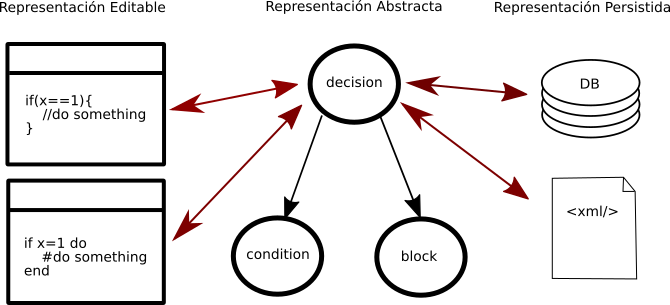
\includegraphics[width=0.5\textwidth,keepaspectratio]{assets/projectional-editor.png}
    \caption{Representaciones de un programa en un editor proyectivo}
  \end{center}
\end{wrapfigure}

A su vez, la \textit{representación abstracta} puede persistirse de diferentes maneras a diferentes soportes, con lo cual se introduce la idea de \textit{representación persistida} para hablar del formato en que guardará el programa, ya sea en una base de datos, un archivo binario, un texto con formato XML, etc.


Esto tiene varias consecuencias:
\begin{itemize}
  \item Deja de necesitarse un parser para el lenguaje, volviéndolo más sencillo de extender.
  \item El programador trabaja más cerca de los conceptos que quiere expresar.
  \item Reduce drásticamente los posibles errores de sintaxis.
  \item El editor trabaja directamente con las instancias de los conceptos, con lo cual:
  \begin{itemize}
    \item es más sencillo analizar el programa
    \item se simplifica la construcción de herramientas (ej: refactors, migrado de versiones de lenguaje, intentions, etc)
    \item se mejora la performance del editor al eliminarse la etapa de parseo.
  \end{itemize}
\end{itemize}


\subsection{MPS Workbench}

MPS (Meta programming System)\cite{MPS} es un ambiente de trabajo orientado al desarrollo de lenguajes específicos de dominio, de la empresa JetBrains, basado en las ideas de Fowler; hoy en día se posiciona como uno de los referentes más importantes en editores proyectivos\cite{LanguageModularity}. 
Entre los productos desarrollados utilizando MPS se encuentran: \textit{MetaR} \cite{MetaR}, un ambiente especializado en biomedicina computacional; \textit{mbeddr} \cite{mbeddr}, un ambiente orientado a software embebido.

\section{Motivación}

En el libro \textit{"Las bases conceptuales de la Programación. Una nueva forma de aprender a programar"}\cite{Gobstones} se presenta una secuencia didáctica bien detallada junto con el entorno \textit{PyGobstones}\cite{PyGobstones}. Sin embargo notamos que, en el marco de una adopción cada vez mayor de esta secuencia didáctica, aparecen nuevas necesidades que el entorno actual no cubre o cubre solo parcialmente:

\begin{itemize}
  \item Disponer de un ambiente que sea facilmente extensible y posea una arquitectura que agilice la colaboración de la comunidad de Gobstones.
  \item Utilizar tecnologías que posean un buen soporte.
  \item Que el entorno sea sencillo de instalar.
  \item Que el entorno constituya un refuerzo de la se secuencia didáctica, y no sólo una herramienta de edición.
  \item Que se encuentre cosntruido sobre soluciones probadas y usadas, en lugar de implementar todos sus componentes desde cero.
\end{itemize}


\section{Propuesta}

Se propone desarrollar un \ile centrado en el lenguaje Gobstones. Para ello se utilizará \textit{MPS Workbench}, cubriendo las necesidades mencionadas en la sección anterior:

\begin{itemize}
  \item soporta tanto extensión de lenguaje como extensión del entorno mediante la creación de plugins.
  \item los features de lenguaje pueden ser activados y desactivados durante el uso del entorno para cumplir con la secuencia didáctica.
  \item es soportado por JetBrains, uno de los líderes mundiales en desarrollo de entornos de programación.
  \item el entorno sólo necesita Java Runtime Environment (siendo que se trabajará sobre la implementación de un intérprete Gobstones, con lo cual se vuelve innecesario contar con un compilador).
\end{itemize}

Entendemos que naturaleza proyectiva de \textit{MPS} cataliza ciertas características deseables en un \ile:

\begin{itemize}
  \item permite al alumno concentrarse en el concepto que desea expresar al reducir notablemente los posibles errores de sintaxis.
  \item el programa siempre se presenta al alumno con un formato estándar (bien indentado, secciones organizadas, etc), ayudándolo a incorporar más rápidamente estas buenas prácticas al reconocerlas como algo natural. En otras palabras, el alumno no posee de antemano una noción de estilos \textit{correctos}, sino que se construye a medida que es expuesto a estos.
\end{itemize}



En particular, de desea que el \ile posea las siguientes características:

\begin{itemize}
  \item una implementación de Gobstones
  \item que incluya la idea de proyecto y ejercicio como mecanismos de organización de código.
  \item que permita limitar los features de lenguaje que pueden ser usados para resolver cierto ejercicio.
  \item que reconozca la especificación del propósito y precondición de funciones y procedimientos (que no sean un comentario más en el código).
  \item que el alumno programe sobre un editor proyectivo
  \item que provea autocompletado, atajos de teclado y navegación de código entre otras funcionalidades comunmente encontradas en editores (siempre y cuando no vayan en contra de la estrategia didáctica)
  \item que provea un mecanismo de integración con otras herramientas que puedan desarrollarse en el futuro, mediante la creación de plugins.
\end{itemize}


\section{Plan de trabajo}

Se organiza el desarrollo en sprints con duración de dos semanas.

\begin{itemize}
  \item{Sprint 1} Modelo puro de Gobstones. Editor que soporte comandos básicos (\textit{Poner}, \textit{Sacar}, \textit{Mover}) y procedimientos sin parámetros.
  \item{Sprint 2} Que el ditor soporte procedimientos con parámetros, variables, ciclos, expresiones booleanas y aritméticas.
  \item{Sprint 3} Se comienza el intérprete del lenguaje. Generación de un tablero a partir de comandos básicos.
  \item{Sprint 4} Soporte a nivel lenguaje para los tableros iniciales. Se concluye el intérprete del lenguaje. 
  \item{Sprint 5} Subproyecto de deploy, generación del entorno. Se agrega soporte para estructura de proyecto y ejercicio.
  \item{Sprint 6} Ejercicios configurables con nivel de lenguaje.
\end{itemize} 



